
\chapter{آزمایش‌ها و نتایج}
\label{ch:results}

این فصل نتایج اندازه‌گیری‌شده را ارائه می‌کند. برای هر نتیجه، سه چیز
مشخص شده است: مقدار مشاهده‌شده، مخرج و شرایط اندازه‌گیری، و
«مرز ادعای مجاز» بر پایه کلاس شواهد آن
(جدول~\ref{tab:evidence-classes}). همه اعداد این فصل از مصنوعات ثبت‌شده و
درهم‌سازی‌شده پروژه خوانده شده‌اند و هیچ مقداری تخمینی نیست.

\section{پوشش شروط پذیرش و وضعیت شواهد}
\label{sec:res-gates}

جدول~\ref{tab:gates} وضعیت شواهد شروط پذیرش پروژه را، همان‌طور که
تجمیع‌کننده شکست‌بسته تولید کرده است، نشان می‌دهد. پنج شرط از نه شرط
شواهد کافی دارند و برای چهار شرط شواهد تکمیلی لازم است. این وضعیت به
کفایت شواهد هر شرط مربوط است و نباید با آمادگی خود گزارش برای ارائه و
داوری یکسان دانسته شود.

\begin{table}[ht]
\centering
\caption{پوشش شروط پذیرش پروژه در تاریخ تولید مصنوع تجمیعی}
\label{tab:gates}
\small
\begin{tabular}{L{8.2cm}c}
\toprule
\textbf{شرط پذیرش} & \textbf{وضعیت شواهد} \\
\midrule
نمونه اولیه کارکردی گفتار‌به‌گفتار فارسی & کافی \\
عبور از آزمون نهایی معنایی خودکار & کافی \\
خروجی ممیزی‌شده در بازه \N{100} تا \N{200} ساعت & کافی \\
حل‌شدن سیاست داده تحت انصراف مستند بازبینی & کافی \\
انتخاب مجوز کد منبع & کافی \\
\midrule
مدل مستقیم فارسی واجد شرایط استقرار & نتیجه مثبت تازه لازم است \\
آشکارساز با دقت بیش از \N{80} درصد روی برچسب مستقل & شواهد تکمیلی لازم است \\
تناسب و تأخیر زنده روی سخت‌افزار \N{12} تا \N{24} گیگابایتی & شواهد تکمیلی لازم است \\
تکمیل مطالعه انسانی & شواهد تکمیلی لازم است \\
\bottomrule
\end{tabular}
\end{table}

\مرزادعا{پنج شرط مهندسی شواهد کافی دارند. چهار ردیف پایانی هنوز به نتیجه
مثبت یا شواهد رسمی تکمیلی نیاز دارند؛ گزارش این فاصله‌ها را صریحاً
به‌عنوان محدودیت و کار آینده ارائه می‌کند و برای نتایج اثبات‌نشده ادعای
قطعی نمی‌سازد.}

\section{مجموعه داده}
\label{sec:res-data}

جدول~\ref{tab:corpus} مشخصات نهایی مجموعه داده را نشان می‌دهد.

\begin{table}[ht]
\centering
\caption{مشخصات مجموعه داده مکالمه فارسی مشتق‌شده و ممیزی خودکار آن}
\label{tab:corpus}
\small
\begin{tabular}{L{7.4cm}R{3.4cm}}
\toprule
\textbf{شاخص} & \textbf{مقدار} \\
\midrule
موجودی زیرنویس کانال‌ها & \N{775.887} ساعت \\
برنامه‌های بلند موجودی & \N{1,442} \\
برنامه‌های انتخاب‌شده & \N{309} \\
پنجره‌های نامزد & \N{1,129} \\
ساعت نامزد پس از انتخاب & \N{219.946} ساعت \\
ساعت چند‌گویندگی طبقه‌بندی‌شده خودکار & \N{207.154} ساعت \\
\midrule
جفت‌های پاسخ بدون بازاستفاده & \N{6,754} \\
ساعت صوت منبع جفت‌ها & \N{123.796} ساعت \\
گویندگان & \N{407} \\
نشست‌ها & \N{162} \\
\midrule
جفت‌های خروجی استریو & \N{6,754} \\
ساعت استریوی خروجی & \N{108.584} ساعت \\
تفکیک آموزش / اعتبارسنجی / آزمون & \N{6,419/131/204} \\
نشت گروهی & \N{0} \\
پرونده‌های گم‌شده در ممیزی & \N{0} \\
شکست ممیزی خودکار & \N{0} \\
\midrule
نامزدهای خودکار رخداد تعاملی & \N{770} \\
از آن، وقفه‌مانند / بازخورد‌مانند & \N{717/53} \\
ردیف‌های تأییدشده توسط انسان & \N{0} \\
\bottomrule
\end{tabular}
\end{table}

مقدار \N{108.584} ساعت درون بازه \N{100} تا \N{200} ساعت نیازمندی ن۴ قرار
می‌گیرد و ممیزی خودکار یکپارچگی، شامل بررسی ترتیب کانال‌ها، درهم‌سازی
پرونده‌ها و تفکیک گروهی، بدون شکست گذشته است.

\مرزادعا{این نتیجه، یک خروجی ممیزی‌شده «خودکار» است. برچسب‌های تعاملی
نامزد خودکارند و شمار ردیف‌های تأییدشده انسانی صفر است؛ بنابراین این
مجموعه داده را نمی‌توان «برچسب‌گذاری‌شده توسط انسان» نامید. همچنین
داده منبع قابل بازنشر نیست.}

\section{سامانه آبشاری: پنل مکانیکی}
\label{sec:res-cascade}

پنل اعتبارسنجی، ۹ ردیف با فاصله ثابت از فهرست‌نامه \N{131} ردیفی
اعتبارسنجی است. شاخص این ردیف‌ها پیش از اجرا قفل شده بود. زنجیره
اجرا‌شده، سرویس واقعی بازشناسی گفتار، پاسخ‌گوی محلی
\en{Qwen2.5-0.5B-Instruct} و موتور گفتاری واقعی است و کانال ورودی، کانال
یک ممیزی‌شده کاربر است. این پنل مکانیک زنجیره را می‌سنجد و نه کیفیت
معنایی پاسخ‌گوی \en{Qwen3-4B} سامانه تحویل‌شده. نتیجه تجمیعی این پنل در
جدول~\ref{tab:cascade-panel} آمده است.

\begin{table}[ht]
\centering
\caption{نتیجه پنل ثابت اعتبارسنجی سامانه آبشاری}
\label{tab:cascade-panel}
\small
\begin{tabular}{L{7.6cm}R{3.2cm}}
\toprule
\textbf{شاخص} & \textbf{مقدار} \\
\midrule
ردیف‌های فهرست‌نامه اعتبارسنجی & \N{131} \\
واحد تفکیک & شناسه نشست منبع \\
نشت تفکیک & \N{0} \\
ردیف‌های ارزیابی‌شده ازپیش‌تعریف‌شده & \N{9} \\
پاسخ‌گوی متنی پنل & \en{Qwen2.5-0.5B-Instruct} \\
\midrule
ردیف‌های عبور‌کرده از همه شروط & \N{9/9} \\
ردیف‌های با پاسخ جایگزین قاعده‌محور & \N{0/9} \\
ردیف‌های با تلاش دوباره زبانی & \N{0/9} \\
خطای سرویس بازشناسی & \N{0} \\
شکست بارگذاری یا تولید مدل زبانی & \N{0/9} \\
کمینه سهم نویسه فارسی در رونویسی & \N{1.000} \\
کمینه سهم نویسه فارسی در پاسخ & \N{1.000} \\
پاسخ‌های صوتی غیرساکت & \N{9/9} \\
کمینه ریشه میانگین مربعات صوت پاسخ & \N{0.133529} \\
ردیف‌های آزمون نهایی استفاده‌شده & \N{0} \\
\bottomrule
\end{tabular}
\end{table}

جدول~\ref{tab:cascade-rows} جزئیات هر ردیف را نشان می‌دهد. ستون زمان،
مدت «تولید کامل پاسخ» است و نه تأخیر نخستین صوت.

\begin{table}[ht]
\centering
\caption{اندازه‌گیری‌های هر ردیف پنل اعتبارسنجی سامانه آبشاری}
\label{tab:cascade-rows}
\small
\begin{tabular}{rrrrrc}
\toprule
\textbf{ردیف} & \textbf{نویسه} & \textbf{مدت صوت} &
\textbf{ریشه میانگین} & \textbf{زمان تولید} & \textbf{عبور} \\
\textbf{فهرست‌نامه} & \textbf{رونویسی} & \textbf{پاسخ (ثانیه)} &
\textbf{مربعات} & \textbf{کامل (ms)} & \\
\midrule
\N{0}   & \N{35}   & \N{4.644} & \N{0.184925} & \N{4895.3}  & بله \\
\N{16}  & \N{541}  & \N{5.352} & \N{0.162841} & \N{5473.7}  & بله \\
\N{32}  & \N{5031} & \N{7.535} & \N{0.210650} & \N{13270.2} & بله \\
\N{48}  & \N{1237} & \N{9.857} & \N{0.191641} & \N{7414.3}  & بله \\
\N{65}  & \N{445}  & \N{9.288} & \N{0.162643} & \N{6664.3}  & بله \\
\N{81}  & \N{2398} & \N{7.465} & \N{0.133529} & \N{12709.4} & بله \\
\N{97}  & \N{77}   & \N{3.448} & \N{0.193290} & \N{2072.4}  & بله \\
\N{113} & \N{405}  & \N{5.259} & \N{0.191777} & \N{3674.2}  & بله \\
\N{130} & \N{142}  & \N{8.824} & \N{0.154569} & \N{5584.7}  & بله \\
\bottomrule
\end{tabular}
\end{table}

یک تحلیل توصیفی پس‌نگر و حریم‌خصوصی‌محور نیز روی همین گزارش اجرا شد که
تنها مقادیر تجمیعی و درهم‌سازی‌ها را می‌خواند و متن رونویسی یا پاسخ را
نمی‌خواند و منتشر نمی‌کند. یافته‌های آن چنین است: هیچ شکست مکانیکی رخ نداد؛
میانه، صدک نود‌و‌پنجم و بیشینه طول رونویسی \N{445}، \N{3977.8} و \N{5031}
نویسه بود؛ میانه، صدک نود‌و‌پنجم و بیشینه زمان تولید کامل \N{5584.736}،
\N{13045.919} و \N{13270.249} میلی‌ثانیه بود؛ سه ردیف رونویسی بیش از
\N{1000} نویسه داشتند و دو ردیف زمان تولید بیش از \N{10} ثانیه.

مهم‌ترین ریسک مهندسی مشاهده‌شده، رشد زمان تولید کامل با طول ورودی است.
همبستگی پیرسون توصیفی میان طول رونویسی و زمان تولید کامل \N{0.885} است و
بلندترین رونویسی و کندترین نوبت، هر دو ردیف \N{32} بودند.
شکل~\ref{fig:cascade}(الف) این رابطه را نشان می‌دهد.

\begin{figure}[ht]
\centering
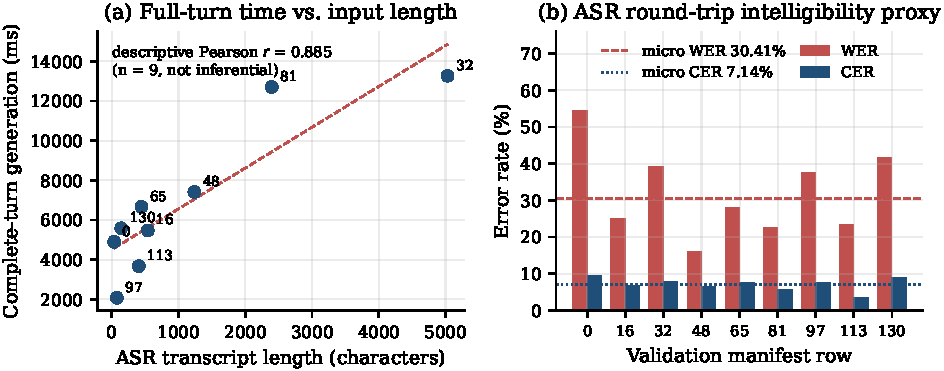
\includegraphics[width=\textwidth]{figs/cascade_panel.pdf}
\caption{(الف) زمان تولید کامل پاسخ در برابر طول رونویسی ورودی برای ۹ ردیف
         پنل اعتبارسنجی، همراه با خط برازش و همبستگی پیرسون توصیفی.
         (ب) نرخ خطای واژه و نویسه بازبازشناسی برای همان ۹ خروجی، همراه با
         مقادیر تجمیع خرد.}
\label{fig:cascade}
\end{figure}

\مرزادعا{این یک نتیجه مثبت مکانیکی و برون‌نمونه روی یک پنل
گروه‌ناهمپوشان با پاسخ‌گوی \en{Qwen2.5-0.5B} است. پنل نه‌ردیفی برای اثبات
تعمیم جمعیتی یا کیفیت معنایی کافی نیست و به پاسخ‌گوی \en{Qwen3-4B} سامانه
تحویل‌شده تعمیم داده نمی‌شود. همبستگی گزارش‌شده توصیفی است و نه استنباطی.
زمان تولید کامل روی سخت‌افزار موجود، سنجه $T_{\text{first\_audio}}$ نیست و
نمی‌تواند شرط \N{500} میلی‌ثانیه را برآورده کند.}

\section{تقریب خودکار فهم‌پذیری گفتار تولیدشده}
\label{sec:res-intel}

برای سنجش این‌که آیا گفتار تولیدشده محتوای متن پاسخ را حفظ می‌کند، یک
اندازه‌گیری بازبازشناسی روی همان ۹ خروجی زنجیره با پاسخ‌گوی
\en{Qwen2.5-0.5B} اجرا شد: متن پاسخ تولیدشده مرجع
است و رونویسی سرویس بازشناسی از موج صوتی خروجی، فرضیه. پروتکل این
اندازه‌گیری، شامل هنجارسازی، تعریف نشانه‌ها و شروط اعتبار، پیش از اجرا ثبت
شده بود و همه درهم‌سازی‌های ورودی بازتولید شدند. نتیجه در
جدول~\ref{tab:intel} گزارش شده است.

\begin{table}[ht]
\centering
\caption{نتیجه تقریب خودکار بازبازشناسی گفتار تولیدشده}
\label{tab:intel}
\small
\begin{tabular}{L{6.8cm}R{4.0cm}}
\toprule
\textbf{شاخص} & \textbf{مقدار} \\
\midrule
ردیف‌های معتبر / خطای سرویس بازشناسی & \N{9/0} \\
\midrule
واژه‌های مرجع / ویرایش‌های واژه & \N{171/52} \\
نرخ خطای واژه تجمیع خرد & \N{30.41\%} \\
نرخ خطای واژه میانگین کلان & \N{32.01\%} \\
نرخ خطای واژه، میانه / صدک ۹۵ / بیشینه &
\N{28.00\%/49.40\%/54.55\%} \\
\midrule
نویسه‌های مرجع / ویرایش‌های نویسه & \N{658/47} \\
نرخ خطای نویسه تجمیع خرد & \N{7.14\%} \\
نرخ خطای نویسه میانگین کلان & \N{7.13\%} \\
نرخ خطای نویسه، میانه / صدک ۹۵ / بیشینه &
\N{7.50\%/9.40\%/9.62\%} \\
\midrule
ردیف‌های با تطابق کامل واژه‌ای & \N{0/9} \\
ردیف‌های با تطابق کامل نویسه‌ای & \N{0/9} \\
\bottomrule
\end{tabular}
\end{table}

شکل~\ref{fig:cascade}(ب) توزیع این دو نرخ خطا را به‌صورت ردیف‌به‌ردیف نشان
می‌دهد. فاصله چشمگیر میان نرخ خطای نویسه و نرخ خطای واژه، در
بخش~\ref{sec:disc-cer-wer} تفسیر شده است.

\مرزادعا{این سنجه یک تقریب خودکار «حفظ محتوا» با یک صدای واحد و روی خروجی
پاسخ‌گوی \en{Qwen2.5-0.5B} است. از آنجا که سرویس بازشناسی هم در سامانه و هم
در اندازه‌گیری مشارکت دارد، و از آنجا که ۹ خروجی برای برآورد فاصله اطمینان
کافی نیست، این نتیجه فهم‌پذیری انسانی، درستی تلفظ، طبیعی‌بودن یا کیفیت
معنایی را اثبات نمی‌کند و به پاسخ‌گوی \en{Qwen3-4B} تعمیم داده نمی‌شود.
هیچ آستانه قبولی نیز پس از مشاهده نتیجه ساخته نشد.}

\section{آزمون معنایی خودکار}
\label{sec:res-semantic}

\subsection{مرحله صلاحیت}

طراحی این ارزیابی دو‌مرحله‌ای است. مرحله نخست روی هفت ردیف
اعتبارسنجی که پیش‌تر استفاده نشده بودند اجرا شد و همه شروط را گذراند:
هر \N{42} فراخوانی داور معتبر بود، میانگین ارتباط نامزد \N{3.857} در برابر
\N{1.000} خط پایه، بهبود ارتباط \N{2.857}، میانگین انسجام \N{3.571} با بهبود
\N{+2.286}، نرخ برد زوجی \N{85.7} درصد (\N{6/7}) و نرخ ارتباط حداقل دو،
\N{100} درصد. تنها پس از این عبور کامل، آزمون نهایی «یک‌بار» باز شد.

\subsection{آزمون نهایی}

آزمون نهایی روی \N{40} ردیف از فهرست‌نامه \N{204} ردیفی آزمون و در پنج
نشست منبع کنارگذاشته اجرا شد. سه بازو به‌صورت دوسوکور و با ترتیب
تصادفی‌شده به داور داده شدند: خط پایه قفل‌شده \en{Qwen2.5-0.5B}، نامزد
\en{Qwen3-4B} با پرامپت \en{v2}، و مرجع هم‌ترازشده خودکار نوبت گوینده
بعدی. داور، مدل \en{Qwen3.8-27B-FP8} با بازنگری
\en{017b9c7af6b5689d5dd426a76e0bc077eb5ca20a}، دمای صفر و دو تکرار در هر
ردیف بود. هر بازو و هر ردیف دو فراخوانی داور برای ارتباط و انسجام دریافت
کرد. جدول~\ref{tab:semantic} نتیجه این آزمون را نشان می‌دهد.

\begin{table}[ht]
\centering
\caption{نتیجه آزمون نهایی معنایی خودکار روی \N{40} ردیف گروه‌ناهمپوشان}
\label{tab:semantic}
\small
\begin{tabular}{L{6.4cm}R{4.4cm}}
\toprule
\textbf{شاخص} & \textbf{مقدار} \\
\midrule
ردیف‌های آزمون & \N{40} \\
نشست‌های منبع & \N{5} \\
فراخوانی معتبر داور / مورد انتظار & \N{240/240} \\
فراخوانی ناموفق داور & \N{0} \\
نرخ توافق تکرار داور & \N{1.00} \\
\midrule
میانگین ارتباط نامزد & \N{3.150} \\
میانگین ارتباط خط پایه & \N{1.425} \\
میانگین ارتباط مرجع هم‌ترازشده & \N{0.950} \\
میانگین انسجام نامزد & \N{3.325} \\
میانگین انسجام خط پایه & \N{1.525} \\
\midrule
بهبود ارتباط نسبت به خط پایه & \N{+1.725} \\
بهبود انسجام نسبت به خط پایه & \N{+1.800} \\
برد زوجی ارتباط & \N{27/40} (\N{67.5\%}) \\
ارتباط حداقل دو & \N{35/40} (\N{87.5\%}) \\
\midrule
تلاش دوباره تولید نامزد & \N{0} \\
صوت نامعتبر نامزد & \N{0} \\
\bottomrule
\end{tabular}
\end{table}

جدول~\ref{tab:semantic-gates} نشان می‌دهد که هر هفت شرط خودکار
ازپیش‌تعریف‌شده برآورده شده‌اند. هیچ آستانه‌ای پس از مشاهده نتیجه تغییر
نکرد.

\begin{table}[ht]
\centering
\caption{شروط خودکار ازپیش‌تعریف‌شده آزمون نهایی و مقادیر مشاهده‌شده}
\label{tab:semantic-gates}
\small
\begin{tabular}{L{5.6cm}rrc}
\toprule
\textbf{شرط} & \textbf{آستانه} & \textbf{مشاهده} & \textbf{وضعیت} \\
\midrule
میانگین ارتباط نامزد & $\ge$ \N{2.00} & \N{3.150} & برآورده \\
میانگین انسجام نامزد & $\ge$ \N{2.50} & \N{3.325} & برآورده \\
بهبود ارتباط & $\ge$ \N{0.50} & \N{1.725} & برآورده \\
بهبود انسجام & $\ge$ \N{0} & \N{1.800} & برآورده \\
نرخ برد زوجی ارتباط & $\ge$ \N{0.60} & \N{0.675} & برآورده \\
نرخ ارتباط حداقل دو & $\ge$ \N{0.70} & \N{0.875} & برآورده \\
اعتبار کامل مکانیکی & \N{240/240} & \N{240/240} & برآورده \\
\bottomrule
\end{tabular}
\end{table}

\مرزادعا{عبور از هفت شرط خودکار به معنای کیفیت ادراکی یا معیار مستقل نیست.
داور و نامزد هم‌خانواده‌اند و این نتیجه در کلاس تقریب خودکار باقی می‌ماند.}

شکل~\ref{fig:semantic} میانگین امتیاز هر بازو و توزیع کامل امتیازها را
نشان می‌دهد. نکته قابل توجه در بخش (ب)، توزیع دو‌قطبی خط پایه است: مدل
\N{0.5} میلیارد‌پارامتری در بخشی از ردیف‌ها امتیاز کامل و در بخش بزرگ‌تری
امتیاز صفر گرفته است. همچنین بازوی مرجع هم‌ترازشده خودکار، پایین‌ترین
امتیاز را دارد؛ تفسیر این مشاهده در بخش~\ref{sec:disc-reference} آمده
است.

\begin{figure}[ht]
\centering
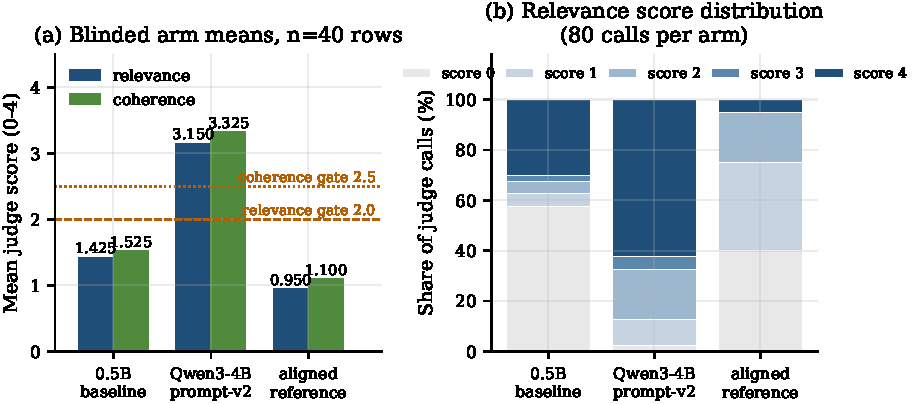
\includegraphics[width=\textwidth]{figs/semantic_final_test.pdf}
\caption{(الف) میانگین امتیاز ارتباط و انسجام برای سه بازوی دوسوکور،
         همراه با آستانه‌های ازپیش‌تعریف‌شده. (ب) توزیع کامل امتیاز ارتباط
         در \N{80} فراخوانی داور برای هر بازو.}
\label{fig:semantic}
\end{figure}

\مرزادعا{این یک نتیجه مثبت «خودکار» با داوری مدل زبانی هم‌خانواده با
نامزد است. ارزیابی انسانی، معیار مستقل گفت‌وگو، سنجش واقعیت یا ایمنی،
اثبات طبیعی‌بودن، تعمیم جمعیتی، تناسب سخت‌افزار هدف و تأخیر مرورگر را
اثبات نمی‌کند.}

\subsection{آزمایش تطبیق پاسخ‌گو با \en{LoRA}}
\label{sec:res-lora}

یک آزمایش جانبی بررسی کرد که آیا تطبیق کم‌پارامتر پاسخ‌گوی متنی روی
نوبت‌های پاسخ همین مجموعه داده، کیفیت معنایی را بهبود می‌دهد. آموزش با
موفقیت اجرا شد و زیان توسعه کاهش یافت: زیان نشانه‌های پاسخ مدل پایه
\N{3.723} بود، پس از دوره نخست \N{2.643} و پس از دوره دوم \N{2.562}، یعنی
\N{31.18} درصد کاهش نسبت به مدل پایه. چک‌پوینت دوره دوم بر پایه کمترین
زیان توسعه انتخاب شد.

اما ارزیابی معنایی روی چهل ردیف آزمون نشان داد که این آداپتر از خط پایه
پیشی نمی‌گیرد. نتیجه به‌عنوان یک «نتیجه منفی معتبر» ثبت شد و آداپتر
در سامانه نهایی به کار نرفت. تفسیر این تناقض ظاهری در
بخش~\ref{sec:disc-reference} آمده است.

\section{تشخیص وقفه}
\label{sec:res-bargein}

\subsection{آزمون مصنوعی}

روی داده مصنوعی، طبقه‌بند تقویت گرادیانی روی \N{32} نمونه کنارگذاشته
(با \N{128} نمونه آموزش) به دقت \N{1.000}، امتیاز \en{F1} کلاس وقفه
\N{1.000}، نرخ پذیرش نادرست \N{0.000} و نرخ رد نادرست \N{0.000} رسید، در
حالی که خط پایه انرژی و نرخ گذر از صفر دقت \N{0.375}، امتیاز \en{F1}
\N{0.545} و نرخ پذیرش نادرست \N{1.000} داشت. فاصله اطمینان ویلسون
\N{95} درصد برای دقت مصنوعی \N{89.28} تا \N{100} درصد است. زمان استنتاج هر گام روی
پردازنده مرکزی \N{7.931} میلی‌ثانیه بود که در بودجه \N{20} میلی‌ثانیه‌ای
هر فریم جای می‌گیرد.

\مرزادعا{دقت کامل روی داده مصنوعی، یک نتیجه معنادار درباره عملکرد واقعی
نیست؛ داده مصنوعی از همان مدل تولیدی ساخته شده که ویژگی‌ها را جدا‌پذیر
می‌کند. این عدد تنها به‌عنوان آزمون بازگشتی نرم‌افزاری ارزش دارد و در این
نوشتار به‌عنوان شاهد کارایی آشکارساز ارائه نمی‌شود.}

\subsection{تقریب روی داده ضبط‌شده}

ارزیابی معنادار روی رخدادهای برگرفته از صوت واقعی مجموعه داده انجام شد.
از \N{1,730} رخداد کشف‌شده، \N{1,048} رخداد انتخاب و بر پایه نشست به سه
بخش تقسیم شد. آستانه تصمیم تنها روی \N{24} نشست اعتبارسنجی انتخاب شد
(مقدار \N{0.70}) و سپس یک‌بار روی \N{22} نشست آزمون با \N{132} رخداد
اعمال گردید. نتیجه در جدول~\ref{tab:bargein} آمده است.

\begin{table}[ht]
\centering
\caption{نتیجه تقریب آشکارساز وقفه روی رخدادهای صوت ضبط‌شده با نشست‌های
         کنارگذاشته}
\label{tab:bargein}
\small
\begin{tabular}{L{3.3cm}rrl}
\toprule
\textbf{سنجه} & \textbf{آشکارساز} & \textbf{خط پایه} &
\textbf{فاصله اطمینان \N{95\%} آشکارساز} \\
 & \textbf{پیشنهادی} & \textbf{انرژی} & \textbf{(بلوکی در سطح نشست)} \\
\midrule
دقت & \N{81.06\%} & \N{78.03\%} & \N{74.44\% -- 87.18\%} \\
امتیاز \en{F1} وقفه & \N{78.99\%} & \N{71.84\%} & \N{72.34\% -- 85.71\%} \\
نرخ پذیرش نادرست & \N{9.09\%} & \N{0.00\%} & \N{2.63\% -- 16.92\%} \\
نرخ رد نادرست & \N{28.79\%} & \N{43.94\%} & \N{19.30\% -- 37.23\%} \\
\bottomrule
\end{tabular}
\end{table}

ماتریس درهم‌ریختگی آشکارساز پیشنهادی روی مجموعه آزمون چنین است: \N{60}
منفی درست، \N{6} مثبت نادرست، \N{19} منفی نادرست و \N{47} مثبت درست.
فاصله اطمینان ویلسون \N{95} درصد در سطح رخداد برای دقت
\N{73.53\%} تا \N{86.83\%}، برای نرخ پذیرش نادرست \N{4.23\%} تا
\N{18.45\%} و برای نرخ رد نادرست \N{19.27\%} تا \N{40.64\%} است؛ فاصله
امتیاز \en{F1} در همین سطح، خودراه‌انداز رخدادی است
(\N{69.47\%} تا \N{86.33\%}). شکل~\ref{fig:bargein} جست‌وجوی آستانه روی نشست‌های اعتبارسنجی و مقایسه
نهایی با خط پایه را نشان می‌دهد.

\begin{figure}[ht]
\centering
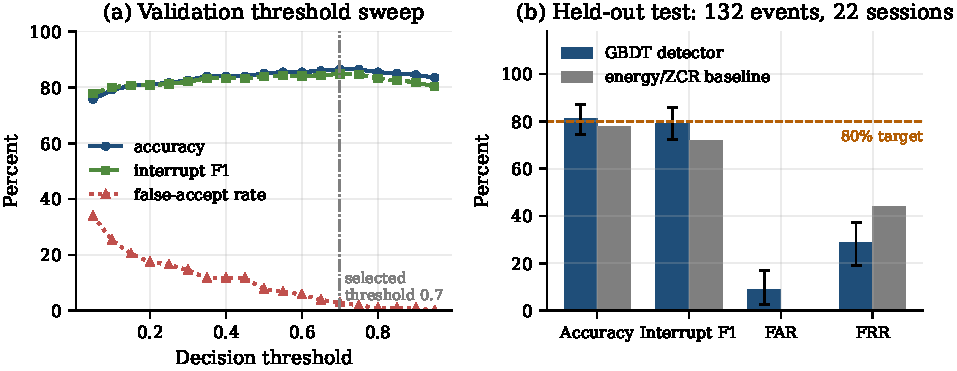
\includegraphics[width=\textwidth]{figs/bargein_proxy.pdf}
\caption{(الف) جست‌وجوی آستانه تصمیم روی نشست‌های اعتبارسنجی؛ خط عمودی،
         آستانه انتخاب‌شده \N{0.70} است. (ب) مقایسه آشکارساز پیشنهادی با
         خط پایه انرژی روی نشست‌های آزمون؛ میله‌های خطا، فاصله اطمینان
         بلوکی در سطح نشست‌اند.}
\label{fig:bargein}
\end{figure}

آشکارساز پیشنهادی در برابر خط پایه، بهبود روشنی در امتیاز \en{F1} کلاس
وقفه و کاهش چشمگیر نرخ رد نادرست نشان می‌دهد. خط پایه انرژی نرخ پذیرش
نادرست صفر دارد اما این به بهای رد \N{43.94} درصد از وقفه‌های واقعی به دست
آمده است، که در یک سامانه تعاملی به معنای بی‌اعتنایی مکرر به کاربر است.

\مرزادعا{دقت نقطه‌ای \N{81.06} درصد از \N{80} درصد بالاتر است، اما کران
پایین فاصله اطمینان بلوکی در سطح نشست \N{74.44} درصد است و از \N{80} درصد
پایین‌تر می‌رود. مهم‌تر آن‌که برچسب‌های مرجع این ارزیابی، از تفکیک گوینده
خودکار به دست آمده‌اند و بازبینی مستقل انسانی ندارند. بنابراین
نیازمندی ن۵ با این شواهد «اثبات نشده» است.}

\section{پیوستگی انتقال تمام‌دوطرفه}
\label{sec:res-duplex}

آزمون بازگشتی خودکار بستر \en{WebSocket} با چهار آزمون گذشت. این آزمون‌ها
تأیید می‌کنند که پیش‌بافر \N{3,200} نمونه‌ای پیش از وقفه با \N{1,600}
نمونه دریافت‌شده پس از آن ترکیب می‌شود و یک ورودی \N{4,800} نمونه‌ای برای
نوبت بعدی می‌سازد. همچنین دریافت تأیید توقف از کارخواه، تله‌متری شناسه
زمان اجرا، لغو نوبت، اتصال هم‌زمان، اتصال مجدد، جداسازی وضعیت نشست‌ها،
ورودی ناقص یا ساکت، بازیابی از خطای تولید و کمبود حافظه، و حالت
نگه‌داری فقط‌سنجه بدون نوشتن پرونده صوتی پوشش داده شده‌اند.

ممیزی نهایی مخزن نیز \N{206} آزمون موفق با پوشش شاخه‌ای \N{65} درصد
(در برابر حد لازم \N{60} درصد) و بررسی نوع بدون خطا روی \N{49} پرونده را
ثبت کرده است.

\مرزادعا{این شواهد پیوستگی را در سطح انتقال سرور اثبات می‌کنند. اجرای
مرورگر فیزیکی انجام نشده است و اجرای سخت‌افزار هدف نیز انجام نشده است؛
بنابراین نیازمندی ن۲ به‌صورت نرم‌افزاری برآورده و به‌صورت رسمی
اثبات‌نشده باقی می‌ماند.}

\section{مسیر مستقیم: شش نسل آزمایشی}
\label{sec:res-moshi}

\subsection{نتیجه کل}

جدول~\ref{tab:moshi-summary} خلاصه شش نسل آزمایشی را نشان می‌دهد. الگوی
مشترک همه نسل‌ها یکسان است: زیان کاهش می‌یابد و شرط اجرای خودرگرسیو
برآورده نمی‌شود.

\begin{table}[ht]
\centering
\caption{خلاصه شش نسل آزمایشی مسیر مستقیم. ستون «بهترین اجرا» بیشترین
         شمار ردیف عبور‌کرده از ۹ ردیف پنل اجرا در میان همه چک‌پوینت‌های
         آن نسل است.}
\label{tab:moshi-summary}
\small
\begin{tabular}{lrrrrc}
\toprule
\textbf{نسخه} & \textbf{پنجره} & \textbf{نامزد} & \textbf{کمینه} &
\textbf{بهترین} & \textbf{واجد} \\
 & \textbf{(ثانیه)} & & \textbf{زیان} & \textbf{اجرا} & \textbf{شرایط} \\
\midrule
\en{v1}   & \N{20}  & \N{16} & \N{1.402} & \N{0/9} & نه \\
\en{v2}   & \N{100} & \N{20} & \N{1.735} & \N{2/9} & نه \\
\en{v3}   & \N{100} & \N{5}  & \N{1.879} & \N{1/9} & نه \\
\en{v4}   & \N{100} & \N{5}  & \N{1.879} & \N{1/9} & نه \\
\en{v5}   & \N{100} & \N{5}  & \N{1.868} & \N{1/9} & نه \\
\en{v6.2} & \N{12}  & \N{4}  & \N{2.060} & \N{0/9} & نه \\
\bottomrule
\end{tabular}
\end{table}

\مرزادعا{مقادیر کمینه زیان میان نسل‌ها «مستقیماً قابل مقایسه نیستند»،
زیرا پنجره متن، مجموعه اعتبارسنجی و شمار نمونه‌های ارزیابی میان نسل‌ها
تفاوت دارد. برای نسخه \en{v6.2}، زیان روی همان داده آموزشی محاسبه شده و
یک سنجه درون‌نمونه است. این ستون تنها برای نشان‌دادن روند کاهش زیان در هر
نسل آورده شده است.}

شکل~\ref{fig:trials} همین دو محور را در برابر یکدیگر می‌گذارد: کاهش زیان
آفلاین در همه نسل‌ها رخ داده است، اما هیچ نسلی به شرط \N{9} از \N{9}
نرسیده است.

\begin{figure}[ht]
\centering
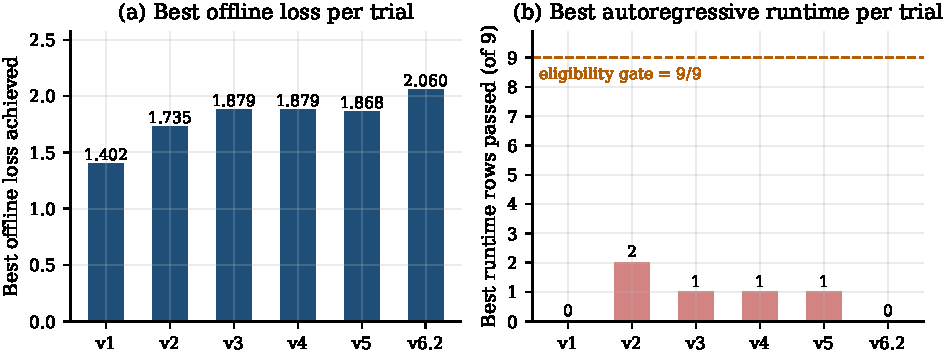
\includegraphics[width=\textwidth]{figs/moshi_trials_summary.pdf}
\caption{(الف) بهترین زیان آفلاین هر نسل. (ب) بیشترین شمار ردیف عبور‌کرده
         از پنل اجرای نه‌ردیفی در هر نسل، در برابر شرط پذیرش
         \N{9} از \N{9}.}
\label{fig:trials}
\end{figure}

\subsection{نسخه نخست: زیان کنارگذاشته مثبت، اجرای ناموفق}

نسخه نخست تا \N{8000} گام و با پنجره \N{20} ثانیه آموزش دید.
شکل~\ref{fig:v1}(الف) روند زیان آموزش و بخش (ب) زیان اعتبارسنجی
بازارزیابی‌شده \N{16} چک‌پوینت را نشان می‌دهد. زیان اعتبارسنجی به‌طور
یکنوا کاهش یافت و چک‌پوینت گام \N{8000} با زیان \N{1.402444} انتخاب شد.

\begin{figure}[ht]
\centering
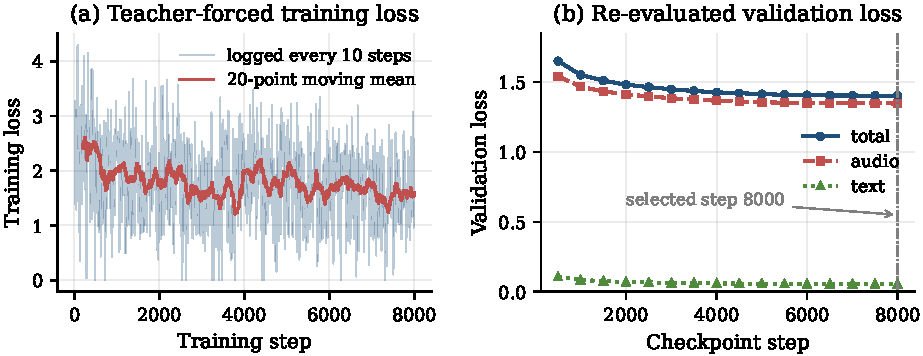
\includegraphics[width=\textwidth]{figs/moshi_v1_training.pdf}
\caption{(الف) زیان آموزش نسخه نخست تحت تحمیل معلم، به همراه میانگین
         غلتان. (ب) زیان اعتبارسنجی بازارزیابی‌شده به تفکیک مؤلفه متنی و
         صوتی؛ خط عمودی، چک‌پوینت انتخاب‌شده است.}
\label{fig:v1}
\end{figure}

روی مجموعه آزمون کنارگذاشته با \N{204} ردیف و \N{331} بازه، این آداپتر
زیان کل \N{1.7272} با فاصله اطمینان \N{95} درصد
\N{1.5866} تا \N{1.8678} داد، در برابر \N{3.5670} برای مدل پایه
تطبیق‌نیافته و \N{9.9871} برای یک گروه کنترل که در آن علامت همه ماتریس‌های
$B$ آداپتر معکوس شده بود. یعنی از دید هدف آموزشی، آداپتر هم نسبت به مدل
پایه و هم نسبت به کنترل، بهبود معنادار داشت.

با این حال، همان آداپتر انتخاب‌شده در سرور جویباری رسمی، صوت تقریباً ساکت و
هیچ متنی تولید نکرد. این تناقض، همان مشاهده‌ای است که تعریف شرط پذیرش
زمان اجرا برای نسل‌های بعدی را ضروری کرد.

\subsection{نسخه دوم: روشن‌ترین نمایش شکاف}

نسخه دوم با پنجره متن \N{100} ثانیه و \N{20} چک‌پوینت نامزد، روشن‌ترین
نمایش الگوی مرکزی این پروژه است. جدول~\ref{tab:v2} چند نقطه از این روند را
نشان می‌دهد و شکل~\ref{fig:v2} تصویر کامل را ارائه می‌کند.

\begin{table}[ht]
\centering
\caption{نمونه‌ای از چک‌پوینت‌های نسخه دوم: زیان اعتبارسنجی به‌طور یکنوا
         کاهش می‌یابد در حالی که شمار ردیف‌های عبور‌کرده از پنل اجرا
         افزایش نمی‌یابد}
\label{tab:v2}
\small
\begin{tabular}{rrrrr}
\toprule
\textbf{گام} & \textbf{زیان کل} & \textbf{زیان متنی} &
\textbf{زیان صوتی} & \textbf{عبور از پنل} \\
\midrule
\N{100}  & \N{2.312407} & \N{0.402789} & \N{1.909618} & \N{0/9} \\
\N{400}  & \N{1.894230} & \N{0.201763} & \N{1.692467} & \N{2/9} \\
\N{800}  & \N{1.792216} & \N{0.164635} & \N{1.627582} & \N{1/9} \\
\N{1000} & \N{1.768085} & \N{0.155691} & \N{1.612394} & \N{1/9} \\
\N{1500} & \N{1.739114} & \N{0.144936} & \N{1.594178} & \N{0/9} \\
\N{2000} & \N{1.734574} & \N{0.143414} & \N{1.591161} & \N{0/9} \\
\bottomrule
\end{tabular}
\end{table}

\begin{figure}[ht]
\centering
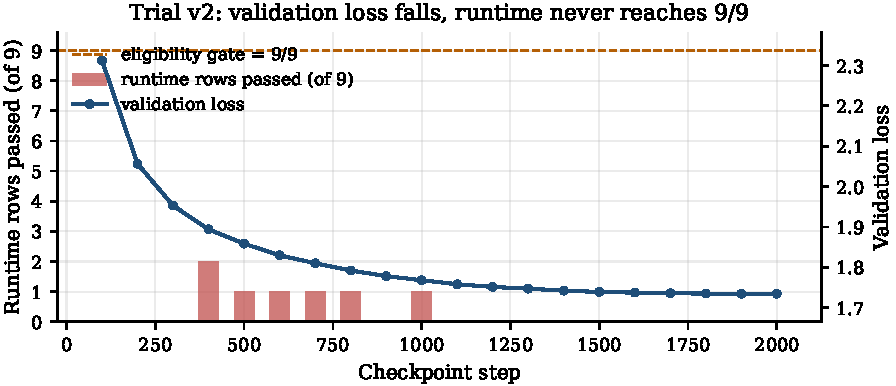
\includegraphics[width=\textwidth]{figs/moshi_v2_loss_vs_runtime.pdf}
\caption{نسخه دوم: زیان اعتبارسنجی روی \N{202} بازه در هر چک‌پوینت به‌طور
         یکنوا کاهش می‌یابد (خط)، در حالی که شمار ردیف‌های عبور‌کرده از پنل
         اجرای نه‌ردیفی (میله‌ها) هرگز به شرط پذیرش نمی‌رسد.}
\label{fig:v2}
\end{figure}

نکته تعیین‌کننده آن است که بهترین رفتار زمان اجرا در گام \N{400} رخ می‌دهد،
یعنی جایی که زیان «بالاتر» است، و با ادامه کاهش زیان تا گام \N{2000}
رفتار زمان اجرا «بدتر» می‌شود و به صفر می‌رسد. این یعنی زیان
اعتبارسنجی در این تنظیم، حتی همبستگی مثبت با کیفیت تولید ندارد.

\subsection{نسخه‌های سوم تا پنجم: آزمون فرضیه‌های هدفمند}

سه نسخه بعدی، فرضیه‌های مشخصی را آزمودند (جدول~\ref{tab:moshi-design}).
نسخه سوم همه درج‌گرها را منجمد کرد و رتبه را به \N{128} افزایش داد. نسخه
چهارم تنها دو درج‌گر متنی را آموزش داد و نسخه پنجم ضریب زیان کتاب رمز نخست
را از \N{100} به \N{10} کاهش داد. جدول~\ref{tab:v45} نتیجه ردیف‌به‌ردیف دو
نسخه آخر را نشان می‌دهد.

\begin{table}[ht]
\centering
\caption{نتیجه هر چک‌پوینت نسخه‌های چهارم و پنجم روی پنل اجرای نه‌ردیفی}
\label{tab:v45}
\small
\begin{tabular}{rrrrrrr}
\toprule
& \multicolumn{3}{c}{\textbf{نسخه چهارم}} &
  \multicolumn{3}{c}{\textbf{نسخه پنجم}} \\
\cmidrule(lr){2-4}\cmidrule(lr){5-7}
\textbf{گام} & \textbf{زیان} & \textbf{گفتار} & \textbf{عبور} &
               \textbf{زیان} & \textbf{گفتار} & \textbf{عبور} \\
\midrule
\N{100} & \N{2.082125} & \N{9/9} & \N{1/9} &
          \N{2.082676} & \N{9/9} & \N{0/9} \\
\N{200} & \N{1.948315} & \N{7/9} & \N{0/9} &
          \N{1.943459} & \N{7/9} & \N{0/9} \\
\N{300} & \N{1.899640} & \N{4/9} & \N{0/9} &
          \N{1.889862} & \N{6/9} & \N{0/9} \\
\N{400} & \N{1.881632} & \N{5/9} & \N{1/9} &
          \N{1.870719} & \N{5/9} & \N{1/9} \\
\N{500} & \N{1.879061} & \N{5/9} & \N{0/9} &
          \N{1.867859} & \N{4/9} & \N{1/9} \\
\bottomrule
\end{tabular}
\end{table}

الگوی مشترک این دو جدول قابل توجه است: با کاهش زیان، شمار ردیف‌هایی که
«اصلاً گفتاری» تولید می‌کنند از \N{9} به \N{4} یا \N{5} کاهش
می‌یابد. یعنی مدل هم‌زمان که هدف آموزشی را بهتر برازش می‌کند، در تولید
خودرگرسیو بیشتر به سکوت میل می‌کند. بیشینه حافظه اختصاص‌یافته نسخه چهارم
\N{28.640} گیگابایت بود.

هر سه نسخه با صفر چک‌پوینت واجد شرایط «شکست‌بسته» شدند، هیچ آداپتری
انتخاب نشد و دیوار آتش آزمون نهایی هیچ‌گاه باز نگردید.

\subsection{نسخه ششم: تفکیک ظرفیت از تولید}

نسخه \en{v6.2} یک آزمون ابطال درون‌نمونه است: آموزش و ارزیابی روی همان
\N{32} نمونه. نتیجه، همان‌طور که در جدول~\ref{tab:v62} و
شکل~\ref{fig:v62} آمده است، دو‌بخشی و روشن است.

\begin{table}[ht]
\centering
\caption{نسخه \en{v6.2}: سیگنال یادگیری درون‌نمونه مثبت در برابر نتیجه
         اجرای خودرگرسیو منفی}
\label{tab:v62}
\small
\begin{tabular}{rrrrc}
\toprule
\textbf{گام} & \textbf{زیان کل} & \textbf{زیان متنی} &
\textbf{زیان صوتی} & \textbf{عبور از پنل} \\
\midrule
\N{50}  & \N{2.636405} & \N{0.812474} & \N{1.823931} & \N{0/9} \\
\N{100} & \N{2.245344} & \N{0.638987} & \N{1.606357} & \N{0/9} \\
\N{150} & \N{2.071542} & \N{0.550852} & \N{1.520690} & \N{0/9} \\
\N{200} & \N{2.060297} & \N{0.551183} & \N{1.509114} & \N{0/9} \\
\bottomrule
\end{tabular}
\end{table}

\begin{figure}[ht]
\centering
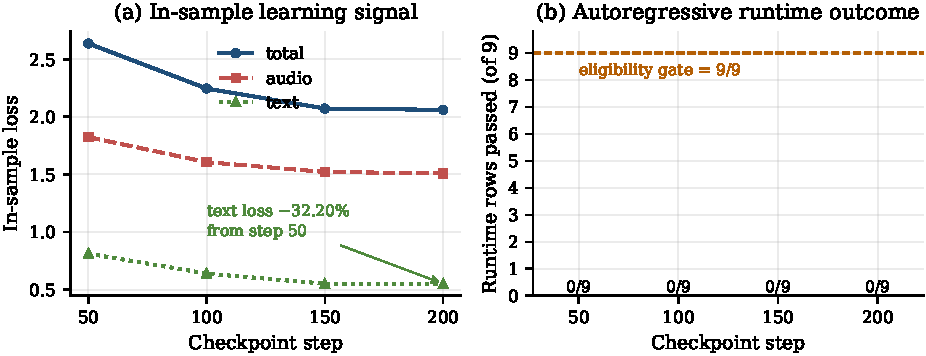
\includegraphics[width=\textwidth]{figs/moshi_v62_diagnostic.pdf}
\caption{نسخه \en{v6.2}: (الف) زیان درون‌نمونه به‌طور پیوسته کاهش می‌یابد و
         کاهش زیان متنی از گام \N{50} به بهترین گام بعدی \N{32.20} درصد
         است. (ب) با این حال هر چهار چک‌پوینت \N{0} از \N{9} ردیف پنل اجرا
         را می‌گذرانند.}
\label{fig:v62}
\end{figure}

بهترین زیان متنی پس از گام \N{50} برابر \N{0.550852} است که \N{32.20}
درصد کمتر از مقدار گام \N{50} (\N{0.812474}) و بالاتر از معیار
ازپیش‌تعریف‌شده \N{30} درصد است. یعنی این آداپتر «ظرفیت» برازش هدف
آموزشی را دارد.

در همان حال، هر چهار چک‌پوینت \N{0} از \N{9} ردیف پنل اجرا را می‌گذرانند و
در هر چک‌پوینت تنها یک ردیف از نه ردیف هم‌زمان متن و گفتار تولید می‌کند.
نتیجه‌گیری دقیق چنین است:

\begin{quote}
نسخه \en{v6.2} هدف آموزشی محدود درون‌نمونه را آموخت، اما رفتار
آموخته‌شده به تولید خودرگرسیو قابل اتکای گفتار و متن فارسی منتقل نشد.
\end{quote}

\مرزادعا{هیچ چک‌پوینتی از هیچ‌یک از شش نسل، واجد شرایط استقرار نیست و هیچ
آزمون نهایی برای مسیر مستقیم باز نشد. عبارت «مدل \en{Moshika} با موفقیت
برای فارسی تنظیم شد» با این شواهد «نادرست» است. نتیجه صحیح، «آزمایش
منفی با سیگنال یادگیری مثبت» است.}

\section{تأخیر و سخت‌افزار}
\label{sec:res-latency}

سخت‌افزار در دسترس پروژه یک پردازنده گرافیکی \en{H100 NVL} با
\N{93.09} گیگابایت حافظه بود، که در بازه \N{12} تا \N{24} گیگابایت
نیازمندی ن۶ قرار نمی‌گیرد. دو آزمون تأخیر سمت سرور اجرا شد:
یکی با سقف نرم‌افزاری \N{24} گیگابایت و یکی بدون سقف. مقادیر
اندازه‌گیری‌شده در جدول~\ref{tab:latency} آمده است.

\begin{table}[ht]
\centering
\caption{اندازه‌گیری‌های تأخیر سمت سرور. این مقادیر کلاس شواهد
         «مؤلفه سمت سرور» دارند و رسمی نیستند.}
\label{tab:latency}
\small
\begin{tabular}{L{3.6cm}rrrc}
\toprule
\textbf{آزمون} & \textbf{تعداد} & \textbf{میانه} & \textbf{صدک ۹۵} &
\textbf{رسمی} \\
 & & \textbf{(ms)} & \textbf{(ms)} & \\
\midrule
نخستین صوت، با سقف حافظه & \N{16} & \N{60.24} & \N{121.87} & نه \\
نخستین صوت، بدون سقف & \N{16} & \N{44.81} & \N{80.26} & نه \\
توقف پخش، با سقف حافظه & \N{16} & \N{17.71} & \N{18.21} & نه \\
توقف پخش، بدون سقف & \N{16} & \N{11.71} & \N{16.02} & نه \\
\midrule
ردیف‌های رسمی سرتاسری & \N{0} & \ناموجود & \ناموجود & \ناموجود \\
\bottomrule
\end{tabular}
\end{table}

\مرزادعا{این مقادیر با صوت مصنوعی و زمان‌سنجی سمت سرور به دست آمده‌اند و
تأیید پخش از سوی مرورگر ندارند؛ همچنین سقف نرم‌افزاری حافظه، یک کارت
\N{93} گیگابایتی را به یک کارت \N{24} گیگابایتی تبدیل نمی‌کند. شمار
ردیف‌های واجد شرایط رسمی سرتاسری «صفر» است. بنابراین ادعای
«تأخیر سامانه کمتر از \N{500} میلی‌ثانیه است» با این شواهد مجاز نیست.
اندازه‌گیری معنادار عملی، همان زمان تولید کامل پاسخ در
جدول~\ref{tab:cascade-rows} است که میانه آن \N{5584.7} میلی‌ثانیه است.}

\section{مطالعه انسانی}
\label{sec:res-study}

پروتکل مطالعه انسانی، شامل سند رضایت‌نامه، برگه امتیازدهی و مجموعه
سناریوهای تعاملی، طراحی و در مخزن ثبت شد. حالت‌های نگه‌داری داده نیز
پیاده شد تا مطالعه بتواند بدون ذخیره پرونده صوتی و تنها با نگه‌داری
بردار ویژگی یا سنجه اجرا شود.

اجرای مطالعه اما تکمیل نشد. وضعیت ثبت‌شده: یک شرکت‌کننده، یک شرکت‌کننده
بالای \N{60} سال، و \N{0} مجموعه امتیاز کامل. مخرج امتیازدهی صفر است و
بنابراین هیچ فاصله اطمینانی قابل برآورد نیست.

\مرزادعا{برای نیازمندی ن۷ شواهد رسمی کافی وجود ندارد. هیچ ادعایی درباره طبیعی‌بودن گفتار
خروجی، رضایت کاربری یا تجربه سالمندان فارسی‌زبان در این نوشتار مطرح
نمی‌شود، و در جداول این فصل هیچ خانه مربوط به ارزیابی انسانی با مقدار
تخمینی پر نشده است.}

\section{وضعیت نهایی نیازمندی‌ها}
\label{sec:res-requirements}

جدول~\ref{tab:req-status} وضعیت هر هفت نیازمندی
جدول~\ref{tab:requirements} را در برابر شواهد به‌دست‌آمده قرار می‌دهد.

\begin{table}[ht]
\centering
\caption{وضعیت نهایی هفت نیازمندی تعریف پروژه و کلاس شواهد پشتیبان}
\label{tab:req-status}
\small
\begin{tabular}{cL{4.0cm}L{5.2cm}}
\toprule
\textbf{شماره} & \textbf{وضعیت} & \textbf{شواهد پشتیبان} \\
\midrule
ن۱ & برآورده برای مسیر آبشاری &
     پنل ثابت \N{9} از \N{9} با صفر پاسخ جایگزین \\
ن۲ & نرم‌افزاری برآورده، رسمی اثبات‌نشده &
     چهار آزمون بازگشتی بستر انتقال؛ بدون مرورگر فیزیکی \\
ن۳ & اندازه‌گیری رسمی انجام نشده &
     صفر ردیف واجد شرایط سرتاسری \\
ن۴ & برآورده &
     \N{108.584} ساعت خروجی ممیزی‌شده، درون بازه هدف \\
ن۵ & پیاده‌سازی‌شده، عبور رسمی اثبات‌نشده &
     دقت \N{81.06\%} با برچسب خودکار؛ کران پایین فاصله اطمینان
     \N{74.44\%} \\
ن۶ & شواهد رسمی موجود نیست &
     سخت‌افزار موجود \N{93.09} گیگابایتی، خارج از بازه هدف \\
ن۷ & شواهد رسمی موجود نیست &
     یک شرکت‌کننده، صفر مجموعه امتیاز کامل \\
\bottomrule
\end{tabular}
\end{table}

\مرزادعا{ن۱ در این جدول تنها عبور مکانیکی \N{9/9} زنجیره با پاسخ‌گوی
\en{Qwen2.5-0.5B} را پوشش می‌دهد. ن۳، ن۵، ن۶ و ن۷ اثبات نشده‌اند؛ ن۵ حتی با
دقت نقطه‌ای \N{81.06} درصد، به‌دلیل برچسب خودکار و کران پایین فاصله اطمینان
نشست، عبور رسمی از \N{80} درصد شمرده نمی‌شود.}

از چهار قلم خروجی مورد انتظار تعریف پروژه، سه قلم تولید و مستند شده‌اند: نمونه
اولیه کارا برای مسیر آبشاری، کد منبع مستند با مجوز آزاد و مجموعه آزمون
خودکار، و مجموعه داده مکالمه فارسی. برای قلم چهارم، پروتکل، رضایت‌نامه و
زیرساخت سنجش آماده است؛ یافته‌های تجربی تعامل سالمندان تنها پس از تکمیل
مطالعه انسانی قابل گزارش خواهد بود و در فصل~\ref{ch:conclusions} به‌عنوان
کار آینده معرفی می‌شود.
